\documentclass[../../General.tex]{subfiles}
\begin{document}


\section{Marco teórico}

El presente marco teórico establece las bases físicas y conceptuales que fundamentan el estudio y justifican la necesidad de una monitorización climática dinámica. Comprender el comportamiento de los sistemas solares frente a las fluctuaciones ambientales es indispensable para evaluar su rendimiento real y superar las limitaciones espaciales que presentan los métodos de medición estáticos convencionales.

\subsection{Fundamentos de la conversión fotovoltaica}
La tecnología fotovoltaica se fundamenta en la conversión directa de la luz solar en electricidad mediante el efecto fotoeléctrico, utilizando como componente central celdas solares de materiales semiconductores, típicamente silicio, estructuradas internamente con una unión P-N, la cual es una unión física de un material semiconductor con huecos positivos (P) y con electrones negativos (N). A nivel físico, la radiación está compuesta por fotones; si la energía de estos impactos supera la banda de energía del material, logran liberar electrones de su estructura atómica. El campo eléctrico intrínseco de la celda se encarga entonces de separar estos portadores de carga, generando un movimiento direccionado que conforma una corriente continua lista para su aprovechamiento, transformación o almacenamiento \citep{martinez2018estimation}.

En la práctica, el rendimiento de esta conversión fotovoltaica no es un valor ideal fijo, sino que fluctúa en función de las condiciones meteorológicas del entorno operativo. Para predecir la potencia efectiva del sistema, se emplea un modelo matemático de estimación. Esta fórmula ajusta la potencia nominal estandarizada de fábrica considerando la cantidad real de luz solar incidente y las pérdidas por estrés térmico:

\begin{equation}
    P_{A} = P_{0} \frac{G_{i}}{1000} C_{K}
\end{equation}

donde:
\begin{itemize}
    \item $P_{0}$: Potencia máxima de instalación en condiciones estándar (W).
    \item $G_{i}$: Irradiancia global en el plano de la instalación ($W/m^{2}$).
    \item $C_{K}$: Factor de ajuste de potencia nominal por temperatura. Sin unidades. Calculado a través de la ecuación.
\end{itemize}

Dado que las condiciones estándar de prueba asumen una temperatura operativa ideal de 25 °C en la celda, el factor $C_{K}$ modela el cambio en la eficiencia cuando el panel tiene una temperatura diferente. Se calcula mediante la siguiente relación:

\begin{equation}
    C_{K} = 1 + \gamma_{P} * (T_{m} - 25)
\end{equation}

donde:
\begin{itemize}
    \item $\gamma_{P}$: Coeficiente relativo de temperatura. Entregado por el fabricante (en $\%.^{\circ}C^{-1}$).
    \item $T_{m}$: Temperatura del panel solar (en $^{\circ}C$).
\end{itemize}


\subsection{Impacto de las variables meteorológicas y pérdidas técnicas}

El rendimiento de los sistemas fotovoltaicos no depende únicamente de sus especificaciones de diseño o fabricación, sino que está condicionado por las variaciones ambientales del entorno en el que operan. Cada instalación posee condiciones climáticas únicas que presentan desafíos diferentes para maximizar la eficiencia energética y optimizar las labores de mantenimiento \citep{chicaiza2024}.


\subsubsection{\textbf{Radiación solar:}} Representa el recurso energético primario. La radiación solar es directamente proporcional a la corriente generada por el panel fotovoltaico. Por lo tanto, cuando la irradiancia sube, la corriente de cortocircuito y la potencia máxima de salida del panel se incrementan \citep{Gonzalez2019Behavioral}. En la Figura \ref{fig:CurvasElectricasIrrTemp} (izquierda), se observa que, para un aumento de 600 a 1000~W/m$^{2}$, el valor de la corriente aumenta en cerca del 88\% para un mismo voltaje.
\subsubsection{\textbf{Temperatura ambiente:}} Influye de manera inversamente proporcional a la eficiencia de conversión debido a las propiedades termodinámicas del material semiconductor. A medida que la temperatura de la celda aumenta, el voltaje de circuito abierto disminuye. Esta caída de tensión provoca una reducción notable en la potencia máxima de salida. Por el contrario, en climas más fríos, la resistencia interna disminuye y el voltaje del panel tiende a aumentar \citep{Gonzalez2019Behavioral}. En la Figura \ref{fig:CurvasElectricasIrrTemp} (derecha), se observa que, para temperaturas de 25 °C y 55 °C, el valor de la potencia disminuye de 225 a 100~W (-55\%),

\begin{figure}[H]

	\captionsetup{justification=raggedright, singlelinecheck=false, labelsep=none}
	
	\caption[Comportamiento eléctrico de un panel solar ante variaciones de irradiancia y temperatura.]{} 
	
	\textit{Comportamiento eléctrico de un panel solar ante variaciones de irradiancia (izquierda) y temperatura (derecha).} \par\medskip
	
	\begin{minipage}{0.5\textwidth}
		\centering
		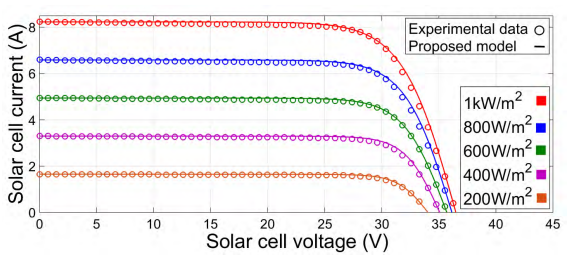
\includegraphics[width=\linewidth]{Recursos/Imagenes/Graficas/IEEE_V_Irr.png}
	\end{minipage}\hfill
	\begin{minipage}{0.5\textwidth}
		\centering
		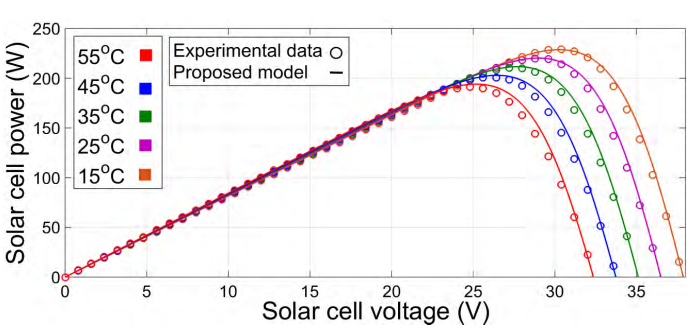
\includegraphics[width=\linewidth]{Recursos/Imagenes/Graficas/IEEE_T_Pwr.png}
	\end{minipage}
	\par\medskip
	
	\raggedright
	\footnotesize \textit{Nota.} Adaptado de \cite{Gonzalez2019Behavioral}.
	\label{fig:CurvasElectricasIrrTemp}
\end{figure}
    
\subsubsection{\textbf{Albedo:}} En el sector fotovoltaico actual, además de los módulos convencionales monofaciales, se emplean cada vez más los paneles bifaciales, los cuales incorporan celdas activas en ambas caras del módulo y son capaces de captar tanto la radiación solar directa en su cara frontal como la radiación reflejada por el suelo en su cara posterior. En este contexto, el albedo, definido como la fracción de luz solar reflejada por la superficie del terreno, adquiere un rol determinante en el rendimiento de estos módulos: un mayor índice de albedo incrementa significativamente la corriente generada en la cara trasera, lo que se traduce en una mayor ganancia bifacial y maximiza la producción total de energía del sistema \citep{Barreno2024}. En la Figura \ref{fig:CurvasElectricasAlbHum} (izquierda), se puede apreciar que, para todo el rango del coeficiente de albedo, la ganancia bifacial aumenta desde 5 a 25\,\%.
    
\subsubsection{\textbf{Humedad y precipitaciones:}} Los altos niveles de humedad relativa provocan la refracción, reflexión y difracción de la luz solar. Esto atenúa la cantidad de radiación directa que logra alcanzar las celdas fotovoltaicas, reduciendo la corriente generada.   En contraste, aunque las precipitaciones reducen la irradiancia momentáneamente, actúan como un mecanismo de mitigación de suciedad al lavar la superficie del panel, removiendo las partículas acumuladas causantes del \textit{soiling} \citep{Kazem2015Humidity}. En la Figura \ref{fig:CurvasElectricasAlbHum} (derecha), se observa que, para una diferencia de humedad del 30\% (entre 95 y 65 \%), el valor de la potencia aumenta de 50 a 105~W (+110\%),

\begin{figure}[H]
	
	\captionsetup{justification=raggedright, singlelinecheck=false, labelsep=none}
	
	\caption[Comportamiento eléctrico de un panel solar ante variaciones de albedo y humedad relativa.]{} 
	
	\textit{Comportamiento eléctrico de un panel solar ante variaciones de albedo (izquierda) y humedad relativa (derecha).} \par\medskip
	
	\begin{minipage}{0.5\textwidth}
		\centering
		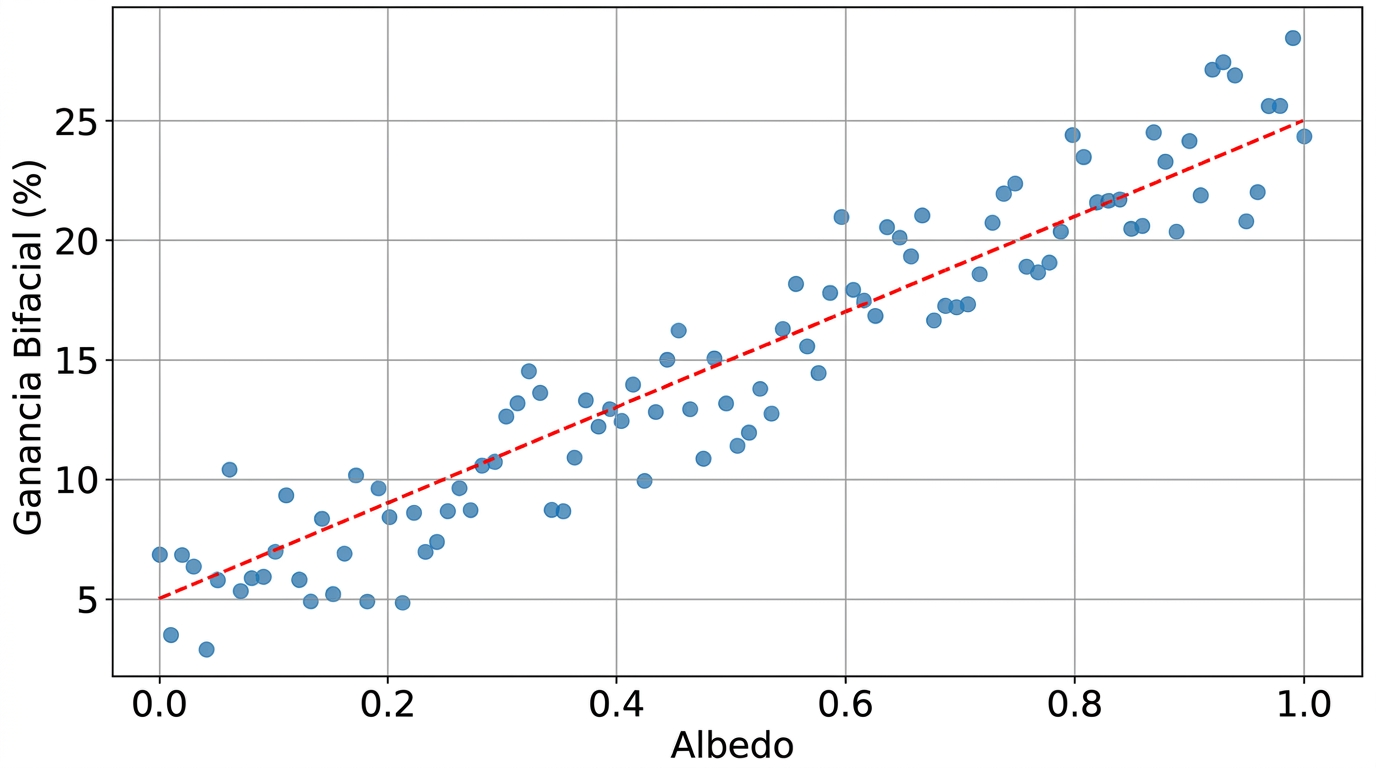
\includegraphics[width=\linewidth]{Recursos/Imagenes/Graficas/BARRENO_Alb_Ganancia.jpeg}
	\end{minipage}\hfill
	\begin{minipage}{0.5\textwidth}
		\centering
		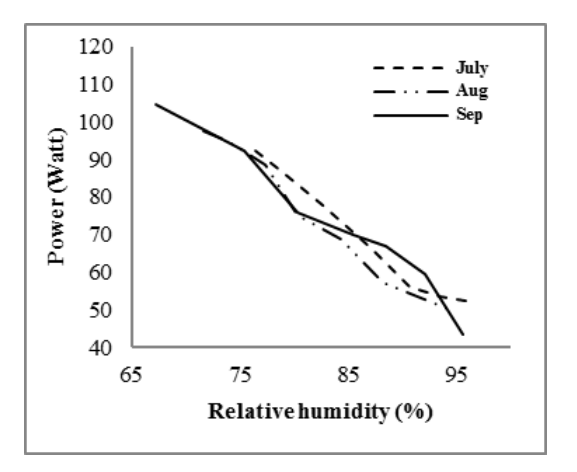
\includegraphics[width=\linewidth]{Recursos/Imagenes/Graficas/KAZEM_Hum_Pwr.png}
	\end{minipage}
	\par\medskip
	
	\raggedright
	\footnotesize \textit{Nota.} Adaptado de \cite{Barreno2024} (izquierda).Adaptado de \cite{Kazem2015Humidity} (derecha).
	\label{fig:CurvasElectricasAlbHum}
\end{figure}


\subsubsection{\textbf{Impacto aerodinámico en topografías complejas:}} El viento presenta un efecto dual. Por un lado, cuando la velocidad del viento es moderada, este favorece el enfriamiento convectivo de los paneles, disipando el calor acumulado y reduciendo la temperatura de la celda, lo que incrementa la eficiencia y la potencia eléctrica de salida. 
Por otro lado, las ráfagas actúan como el principal transporte de partículas. Esto eleva las tasas de deposición de suciedad sobre los cristales, disminuyendo la generación de energía \citep{Vick_WindEffect}. En la Figura \ref{fig:VientoMarcoTeorico} (izquierda), se observa una comparación cualitativa de la potencia de salida de dos paneles solares, con una diferencia promedio a lo largo de día de 7~W (11\% de potencia máxima de panel con aire).

A pesar de la importancia crítica de este enfriamiento convectivo, cuando las plantas a gran escala se instalan sobre terrenos montañosos, las laderas alteran drásticamente el flujo de aire homogéneo. Tal como se evidencia en los contornos de velocidad de la Figura \ref{fig:VientoMarcoTeorico} (derecha) del estudio de \cite{Xu2024}, el relieve actúa como una barrera que estanca el viento en la base de la pendiente, anulando el enfriamiento convectivo, y lo acelera en la cresta. Esta dinámica de fluidos provoca que la capacidad de disipación de calor varíe severamente dependiendo de la elevación exacta de cada panel en el terreno, dando origen a la formación de microclimas.

\begin{figure}[H]
	
	\captionsetup{justification=raggedright, singlelinecheck=false, labelsep=none}
	
	\caption[Comparación entre potencia genera en un panel con o sin viento (izquierda) y efecto de la inclinación de una pendiente en el perfil de velocidad en la base de una ladera de 30° (derecha).]{} 
	
	\textit{Comparación entre potencia genera en un panel con o sin viento (izquierda) y efecto de la inclinación de una pendiente en el perfil de velocidad en la base de una ladera de 30° (derecha).} \par\medskip
	
	\begin{minipage}{0.5\textwidth}
		\centering
		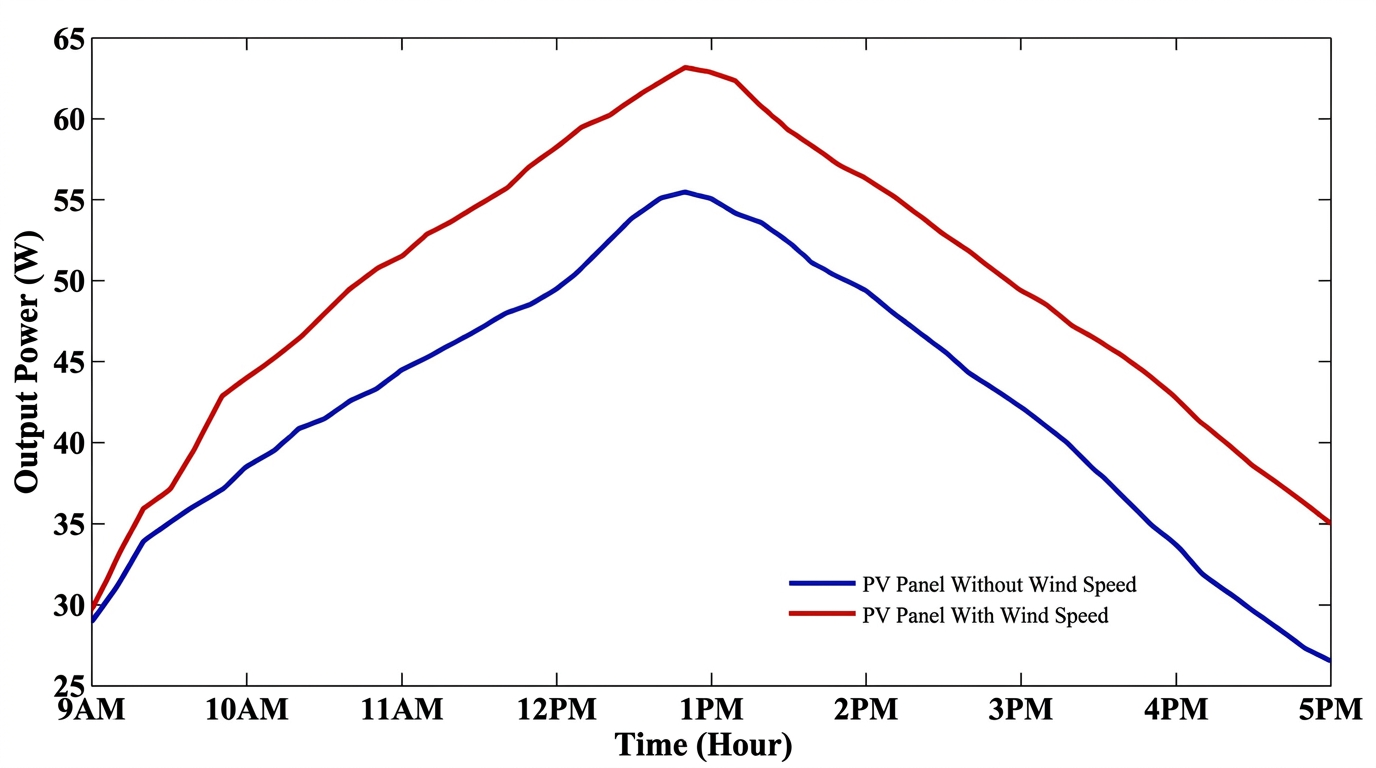
\includegraphics[width=\linewidth]{Recursos/Imagenes/Graficas/Leow_Wind_Pwr.jpeg}
	\end{minipage}\hfill
	\begin{minipage}{0.5\textwidth}
		\centering
		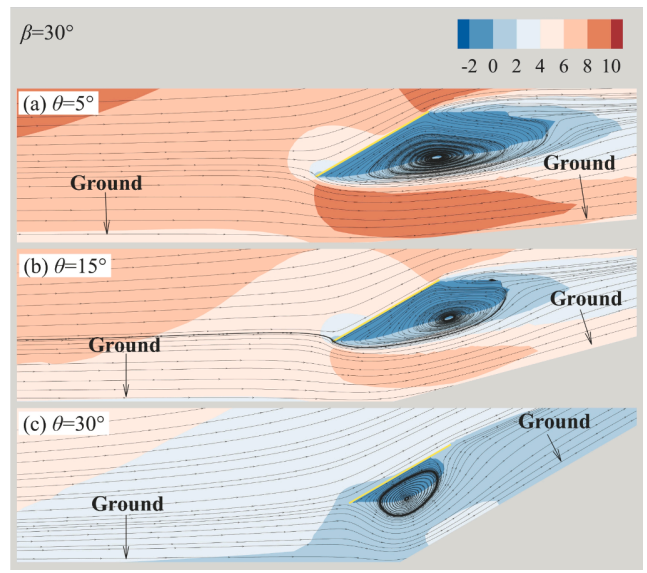
\includegraphics[width=\linewidth]{Recursos/Imagenes/Graficas/XU_Wind_Topography.png}
	\end{minipage}
	\par\medskip
	
	\raggedright
	\footnotesize \textit{Nota.} Adaptado de \cite{Leow2019Wind} (izquierda). Adaptado de \cite{Xu2024} (derecha).
	\label{fig:VientoMarcoTeorico}
\end{figure}




\subsubsection{Formación de microclimas y heterogeneidad espacial}
Las variaciones aerodinámicas generan un enfriamiento desigual en la planta. Al recibir distintos flujos de aire, los paneles experimentan gradientes térmicos considerables; tal como lo demuestra empíricamente el histograma de la Figura \ref{fig:Garcias2014Temp} del estudio de \cite{Garcia2014}, se registran variaciones de temperatura de hasta 7 °C entre módulos separados por 466 y 2716 metros. A este desbalance térmico se suma la variabilidad de la radiación reflejada (albedo) producida por las diferentes inclinaciones del suelo \citep{Salinas2025}. En consecuencia, el rendimiento eléctrico no es uniforme, lo que invalida la premisa de un entorno térmico estable y exige el uso de medición climática dinámica en todo el terreno.

\begin{figure}[H]
	\captionsetup{justification=raggedright, singlelinecheck=false, labelsep=none}
	\caption[Frecuencia anual de las diferencias máximas de irradiancia diaria entre módulos fotovoltaicos por dispersión geográfica.]{} 
	\textit{Frecuencia anual de las diferencias máximas de irradiancia diaria entre módulos fotovoltaicos por dispersión geográfica.} \par\medskip
	
	\centering
	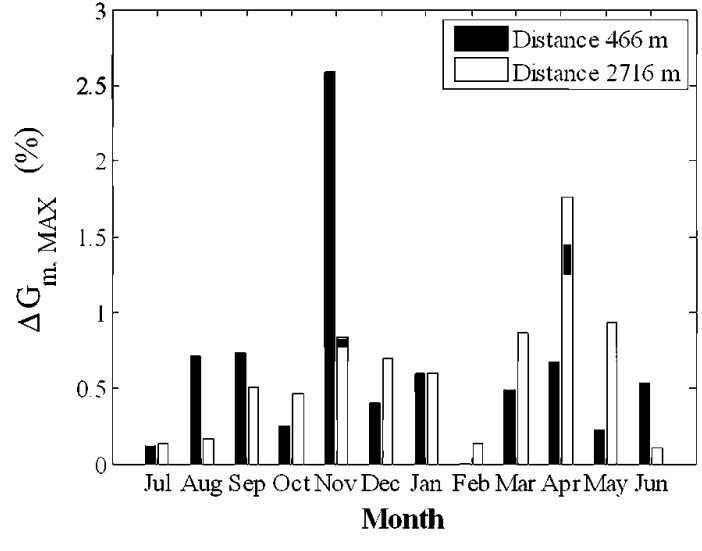
\includegraphics[width=0.6\textwidth]{Recursos/Imagenes/Graficas/GARCIA_Var_Irr.png} \par\medskip
	\raggedright
	\footnotesize \textit{Nota.} Gráfico adaptado del artículo ``Solar irradiation and PV module temperature dispersion
	at a large-scale PV plant'' \citep{Garcia2014}.
	\label{fig:Garcias2014Temp}
\end{figure}

\subsubsection{Pérdidas Técnicas:}

La eficiencia de esta conversión disminuye significativamente bajo condiciones operativas reales debido a dos fenómenos físicos principales. En primer lugar, el efecto térmico provoca que las celdas solares pierdan eficiencia a medida que su temperatura aumenta, ya que dicho incremento genera un coeficiente negativo en el voltaje de circuito abierto que reduce drásticamente la potencia máxima de salida \citep{Vieira2024}. Por otro lado, el fenómeno del \textit{soiling} consiste en la acumulación de polvo, arena y contaminantes sobre la superficie de los módulos; esta capa de suciedad interfiere con la transmisión de la luz mediante procesos de absorción, reflexión y dispersión, generando pérdidas eléctricas que, al distribuirse de forma no uniforme, pueden derivar en la formación de puntos calientes” perjudiciales para la vida útil del panel y reducir severamente la rentabilidad de la instalación \citep{TesisJGB}.


\end{document}
